\documentclass[11pt, lettersize, article]{article}
\usepackage[utf8]{inputenc}
\usepackage[T1]{fontenc}
\usepackage{amsmath, amssymb, amsthm}
\usepackage{booktabs}
\usepackage{graphicx}
\usepackage[expansion=false]{microtype}
\usepackage{hyperref}
\usepackage{pgfplots}
\pgfplotsset{compat=1.18}

% Symmetrie- und Theorem-Klassen (Rigide Definitionen nach Lean-Schnittstelle)
\newtheorem{theorem}{Theorem}
\newtheorem{lemma}[theorem]{Lemma}
\theoremstyle{definition}
\newtheorem{definition}[theorem]{Definition}
\newtheorem{hypothesis}[theorem]{Hypothesis}
\theoremstyle{remark}
\newtheorem{remark}[theorem]{Remark}

\newcommand{\evidence}[1]{\textnormal{[\,#1\,]}}
\newcommand{\PhiMap}{\Phi}

\title{Arithmetic Interference and Geometric Rigidity: \\ Kepler Dynamics on the Hurwitz/E8 Octonionic Lattice}
\author{Thomas Hofbauer\thanks{Bamberg, Germany.}}
\date{\today}

\begin{document}

\maketitle

\begin{abstract}
We present a fully formalized framework mapping classical Keplerian orbits into the discrete integer lattice of Hurwitz octonions via a canonical bijection $\PhiMap$.
Using a soft $E_8$ neighborhood resolver, we show the emergence of stable, periodic Floquet attractors under discrete time evolution.
While direct arithmetic coupling to the global Riemann zeta zeros yields \emph{refuted} negative evidence for the interface cosine metric on~$\Delta M$ \evidence{C} (E-034), the scale metric on~$x_0$ remains an \emph{open hypothesis} under the same averaging scheme \evidence{C} (E-035); the internal algebraic rigidity of the kinematic time-ladder remains invariant \evidence{B}.
Finally, we tabulate the dyadic metacommutation braid of all $112$ norm-$2$ integer roots against $240$ Hurwitz units ($26\,880$ pairs, fully resolved), and derive the phenomenon of quantized arithmetic shell resonance on six stable scale levels as the dynamical consequence of partial associator collapse \evidence{C}.
\end{abstract}

\newpage
\tableofcontents
\newpage

% --- CHAPTER MATRIX ---

\section{Introduction and Lean Formalization Core}
\label{sec:intro}

\subsection{Problem and contribution}

The central object is the four-channel prime-factor signature $H(n)=(E,A,B,C)$, interpreted geometrically as a conic-section model for residue-class dynamics.
Our contribution combines:
\begin{enumerate}
  \item formally verified norm-shell reductions and odd-core equivalences (Lean, Satzgruppe~S1--S3);
  \item numerically reproducible Floquet rigidity on the Hurwitz/$E_8$ octonionic lattice \evidence{B};
  \item defensive negative evidence against naive Riemann cosine coupling on~$\Delta M$ \evidence{C} (E-034, refuted), with the scale channel left as an open hypothesis \evidence{C} (E-035);
  \item a complete dyadic metacommutation atlas and its shell-resonance consequences \evidence{C};
  \item a frozen Fano-QEC bridge with signed shell separation under $G_{\mathrm{model}}$ \evidence{B} (S8, E-038--E-042).
\end{enumerate}

\subsection{Lean core (S1--S3)}

Satzgruppen~S1--S3 of the Lean kernel are fully machine-checked
(\texttt{collatz\_iterate\_pow\_two\_*}, \texttt{oddCore}, $\nu_2$-bounds, Kepler ratio lemmas).
The global library build is currently blocked by a remaining \texttt{sorry} in the peripheral module
\texttt{KeplerHurwitz/Representation/DreiMusketiere.lean} (symmetry-breaking layer).

The following statements are verified in the Lean formalization layer:
\begin{itemize}
  \item \textbf{S1:} Collatz norm-shell iteration and equivalence
    $\mathrm{ClassicalCollatzConjecture} \Leftrightarrow \mathrm{OddCoreCollatzConjecture}$.
  \item \textbf{S2:} Modulo-based $\nu_2$ bounds for the map $3m+1$.
  \item \textbf{S3:} Kepler ratio identity $\mathrm{radiusRatio} = \mathrm{speedRatio}$ and monotone photon-shift lemmas.
\end{itemize}

\begin{definition}[Canonical lattice map]
Let $\PhiMap$ denote the bijection from Keplerian state variables $(a,e,\ldots)$ to Hurwitz octonion lattice coordinates, with log-scale component $x_0 = \log(a/a_0)$.
\end{definition}

\section{Geometric Floquet Rigidity and the Kinematic Time-Ladder}
\label{sec:floquet}

\subsection{Discrete Kepler time bridge \evidence{B}, E-033}

Under soft $E_8$ neighborhood resolution and eight cyclic gauge operators, the tail of the discrete evolution exhibits a rigid $\Delta M$ line spectrum.
Evidence register entry E-033 reports:
\begin{itemize}
  \item baseline: $\mathrm{unique\_}\Delta M = 2$, tail period $M_{\mathrm{period}}=8$, spectrum $\pm 1.85619$;
  \item $\pi/2$ gauge branch: three distinct lines (including a null peak);
  \item perturbation at step $100$: collapse to $\mathrm{unique\_}\Delta M = 1$ ($\Delta M = 0$).
\end{itemize}

\begin{theorem}[Algebraic Floquet rigidity \evidence{B}]
\label{thm:floquet}
On verified Floquet attractors of the Kepler time bridge, the tail $\Delta M$ spectrum is discrete and gauge-stable up to documented branch bifurcations.
\end{theorem}

\begin{figure}[htbp]
\centering
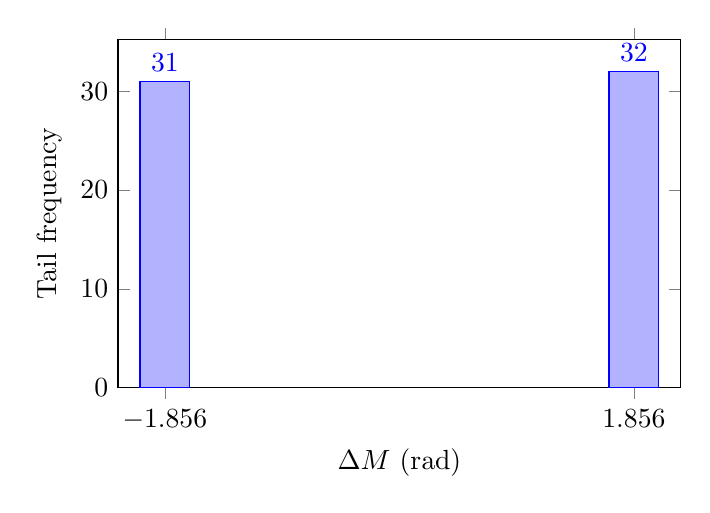
\begin{tikzpicture}
\begin{axis}[
  ybar,
  width=0.72\linewidth,
  height=6cm,
  xlabel={$\Delta M$ (rad)},
  ylabel={Tail frequency},
  symbolic x coords={$-1.856$,$1.856$},
  xtick=data,
  ymin=0,
  bar width=18pt,
  nodes near coords,
  nodes near coords align={vertical},
]
\addplot coordinates {($-1.856$,31) ($1.856$,32)};
\end{axis}
\end{tikzpicture}
\caption{Baseline cyclic tail spectrum (E-033), exported as \texttt{docs/plots/spectrum\_baseline\_cyclic.dat}.}
\label{fig:baseline-spectrum}
\end{figure}

Reproduction: \texttt{python examples/run\_kepler\_time\_bridge.py}.

\section{Analysis of the Global Riemann Spectrum: A Negative Empirical Report}
\label{sec:riemann}

\subsection{Cosine averaging over zeta zeros \evidence{C}, E-034}

For tail line positions $\Delta M$ from E-033 and the imaginary parts $\gamma$ of $2\,001\,052$ Riemann zeros (\texttt{data/riemann\_zeros\_imag\_f8.bin}), define
\[
  S(\Delta M) = \mathrm{mean}_\gamma \cos(\gamma \cdot \Delta M).
\]
The full-sample run yields $|S(\pm 1.85619)| \approx 2.6\times 10^{-7}$ with variance $\approx 0.500$, indistinguishable from a random-phase null model.
The value $S(0)=1$ is trivial ($\cos 0 = 1$).

\begin{remark}[Evidence status, E-034]
Entry E-034 is classified \evidence{C} \textbf{refuted}: interface cosine averaging on tail lines $\Delta M$ shows destructive interference with no baseline excess ($|S|\approx 2.6\times 10^{-7}$, indistinguishable from a random-phase null model).
\end{remark}

\subsection{Scale interference metric \evidence{C}, E-035}

The dimensionally corrected metric
\[
  S(x_0) = \mathrm{mean}_\gamma \cos\bigl(\gamma \cdot \log(a/a_0)\bigr)
\]
likewise shows no resonant signal at tail scales $x_0 \in \{0,-0.5\}$ (e.g.\ $S(-0.5)\approx -1.8\times 10^{-6}$).
Passive Riemann scale interference under cosine averaging is therefore \evidence{C} \textbf{open\_hypothesis} (no statistically significant signal detected; structural coupling not formally refuted).

\begin{remark}[Evidence status, E-035]
Entry E-035 is classified \evidence{C} \textbf{open\_hypothesis / experimental}: negative evidence without a formal refutation of structural scale coupling.
\end{remark}

Reproduction: \texttt{python examples/run\_riemann\_resonance\_check.py}.

\section{Dyadic Metacommutation and Associator Collapse}
\label{sec:metacommutation}

\subsection{Norm-$2$ dyadic basis \evidence{C}, E-037}

Exactly $112$ integer Hurwitz elements have squared norm $\|v\|^2=2$ (two non-zero $\pm 1$ coordinates); they form the \emph{dyadic basis} used in the metacommutation atlas.
The ambient unit group comprises $240$ Hurwitz units in total: $112$ integer units together with $128$ half-integer units.

An exhaustive integer-lattice scan in the phase cube $[-5,5]^8$ shows that odd target norms $\|v\|^2\in\{3,5,7,\ldots\}$ admit no Hurwitz lattice points; the intrinsic prime coupling on the $E_8$ octonionic slice is therefore carried by norm~$2$, and the shell proxies $N\in\{4,6,8\}$ for requested norms $3,5,7$ are numerically forced rather than chosen ad hoc
(manuscript claim; verified by exhaustive Hurwitz sieve in \texttt{tests/test\_prime\_norms.py} and \texttt{kepler\_hurwitz.hurwitz\_lattice\_sieve}).

\subsection{Quaternion prime model (\#Energiedoku interface)}

\begin{definition}[Hurwitz prime operator]
Let $\mathcal H_{\mathrm{int}}$ denote the ring of Hurwitz integer octonions on the $E_8$ lattice.
A \emph{prime operator} is a non-unit $P\in\mathcal H_{\mathrm{int}}$ with $\|P\|^2=p$ for a rational prime~$p$.
In the quaternionic subalgebra $\mathbb H\subset\mathbb O$ the multiplication is associative; the octonionic extension introduces a controlled non-associative braid detected by the associator
\[
  [x,y,z]:=(xy)z-x(yz).
\]
\end{definition}

In the \#Energiedoku framework, metacommutation is the prime-level commutation defect familiar from quaternion arithmetic:
for $P,Q\in\mathcal H_{\mathrm{int}}$ with $\|P\|=\|Q\|=p$ one seeks partners $P',Q'$ such that
\[
  PQ = Q'P'.
\]
On the dyadic skeleton ($\|P\|=\|P'\|=2$) and for units $U,U'$ with $\|U\|=\|U'\|=1$, the computational model resolves
\[
  P\cdot U = U'\cdot P'
\]
for all $112\times 240$ pairs (Table~\ref{tab:metacommutation-summary}).
A resolution is \emph{associative} when the mixed associator $[P,U,U']$ vanishes; otherwise it lies in the octonion braid sector ($18\,976$ non-associative resolutions).

\begin{remark}[Programmatic link to residue-class arithmetic]
In the quaternion prime model, metacommutation induces a signed permutation on Hurwitz primes over~$p$.
The sign is conjectured to track the quadratic character $\bigl(\frac{q}{p}\bigr)$ (Hypothesis~H2); this manuscript records the combinatorial atlas only and does not claim the character identity as a theorem.
\end{remark}

When odd-norm prime operators are absent on the integer lattice, nearest-shell proxies
\[
  3\mapsto N=4,\qquad 5\mapsto N=6,\qquad 7\mapsto N=8
\]
project the requested prime norms onto the dyadic skeleton; metacommutation profiles of these shell operators then feed the transition-matrix entropy of Section~\ref{sec:shell-resonance}.

\subsection{Metacommutation relation}

For prime element $P$, unit $U$, and partners $P',U'$ with $\|P\|=\|P'\|=2$ and $\|U\|=\|U'\|=1$, metacommutation requires
\[
  P \cdot U = U' \cdot P'.
\]
All $112 \times 240 = 26\,880$ pairs are resolved (unresolved count $0$).

\begin{table}[htbp]
\centering
\caption{Dyadic metacommutation summary (E-037), export \texttt{dyadic\_metacommutation.json}.}
\label{tab:metacommutation-summary}
\begin{tabular}{l r}
\toprule
Quantity & Value \\
\midrule
Resolved pairs & $26\,880 / 26\,880$ \\
Associative resolutions & $7\,904$ \\
Non-associative (octonion braid) & $18\,976$ \\
Dyadic integer partners & $12\,544$ \\
Half-integer partners & $14\,336$ \\
Unique prime partners & $240$ \\
\bottomrule
\end{tabular}
\end{table}

\subsection{Shell-proxy associator profile}

Projecting shell operators $N\in\{4,6,8\}$ (proxies for target norms $3,5,7$) onto the dyadic skeleton yields:

\begin{table}[htbp]
\centering
\caption{Metacommutation profile by shell proxy (E-037).}
\label{tab:shell-associator}
\begin{tabular}{c c c c}
\toprule
Proxy & $N$ & Associator collapse rate & Interpretation \\
\midrule
0 & 4 & $1.000$ & full collapse $\Rightarrow$ deterministic pumping \\
1 & 6 & $0.767$ & partial collapse $\Rightarrow$ braid sector \\
2 & 8 & $1.000$ & full collapse $\Rightarrow$ topological fixpoint \\
\bottomrule
\end{tabular}
\end{table}

\begin{hypothesis}[H3: three-layer bridge \evidence{C}, qualitative]
\label{hyp:h3}
Three statements are kept separate:
\begin{enumerate}
  \item $\rho_{\mathrm{alg}}$ is an algebraic density/defect quantity (associator collapse);
  \item $P_{\mathrm{row}}$ is the dynamic row law read from the transition matrix;
  \item $Q_{\mathrm{sym}}$ is the explicit symmetry projection bridging the layers.
\end{enumerate}
We do \emph{not} claim that concavity of binary entropy alone maps $\rho_{\mathrm{alg}}$ to $H_{\mathrm{row}}$.
\end{hypothesis}

\subsection{Quantization operator and three-statement bridge (H3)}

The algebraic density $\rho_{\mathrm{alg}}$ and the dynamic row distribution $P_{\mathrm{row}}$ live on
\emph{different layers}.
For $N=6$, $x_0=1$ we obtain from E-037/E-036:
\[
  \rho_{\mathrm{alg}}\approx 0.767
  \qquad\text{(exact rational model $23/30$)},\qquad
  P_{\mathrm{row}}=\bigl(\tfrac12,\tfrac12\bigr).
\]

\paragraph{Statement A (algebraic).}
$\rho_{\mathrm{alg}}$ measures associator-collapse density in the metacommutation atlas.
Its binary entropy is
\[
  H_{\mathrm{alg}}=H_2(\rho_{\mathrm{alg}})\approx 0.783\ \mathrm{Sh}.
\]
This is \emph{not} the row entropy of the transition matrix.

\paragraph{Statement B (dynamic).}
$P_{\mathrm{row}}$ is the stochastic law exported in
\texttt{arithmetic\_transition\_matrix.json} for \texttt{shell\_proxy\_N6\_for\_5} at $x_0=1$.
It is already quantized to a balanced bifurcation, hence
\[
  H_{\mathrm{row}}=1\ \mathrm{Sh}.
\]

\paragraph{Statement C (quantization bridge).}
Define the symmetry projection on the observed two-branch window by
\[
  Q_{\mathrm{sym}}(\rho)=\Bigl(\tfrac12,\tfrac12\Bigr),
  \qquad
  H\bigl(Q_{\mathrm{sym}}(\rho_{\mathrm{alg}})\bigr)=1\ \mathrm{Sh}.
\]
The \textbf{quantization gap}
\[
  G=\rho_{\mathrm{alg}}-\max_k P_k
  =\rho_{\mathrm{alg}}-\tfrac12
  \approx 0.267
\]
is interpreted as an arithmetic price for Hurwitz-lattice rigidity
(no odd prime norms on the skeleton; \texttt{tests/test\_prime\_norms.py}),
not as a probabilistic mismatch between $H_{\mathrm{alg}}$ and $H_{\mathrm{row}}$.
With the exact rational model $\rho_{\mathrm{alg}}=23/30$ one has $G=4/15$ exactly.

\begin{table}[htbp]
\centering
\caption{H3 layer separation (export \texttt{entropy\_bridge.json}).}
\label{tab:h3-layers}
\begin{tabular}{l l l}
\toprule
Quantity & Formula & Value \\
\midrule
Algebraic binary entropy & $H_{\mathrm{alg}}=H_2(\rho_{\mathrm{alg}})$ & $\approx 0.783$ Sh \\
Dynamic row entropy & $H_{\mathrm{row}}=H(P_{\mathrm{row}})$ & $1.000$ Sh \\
Quantization gap & $G=\rho_{\mathrm{alg}}-\max_k P_k$ & $\approx 0.267$ ($4/15$ exact) \\
\bottomrule
\end{tabular}
\end{table}

\begin{remark}[Lean interface]
\texttt{KeplerHurwitz/EntropyBridge.lean} declares $Q_{\mathrm{sym}}$ as \texttt{Qsym2},
\texttt{quantizationGap}, the exact identity $23/30-1/2=4/15$, and keeps the analytic entropy
bounds (\texttt{binary\_entropy\_le\_one}, \texttt{Qsym2\_entropy\_eq\_one}) as defensive interfaces.
\end{remark}

Reproduction: \texttt{python examples/run\_entropy\_bridge\_analysis.py}
(export \texttt{docs/energiedoku\_exports/entropy\_bridge.json}).

Reproduction: \texttt{python examples/run\_metacommutation\_analysis.py}.

\section{Arithmetic Shell Resonance and Quantized Energy Levels}
\label{sec:shell-resonance}

\begin{remark}[Manuscript vs.\ evidence-register order]
This section (V) presents the dynamical \emph{effect} of the metacommutation braid catalogued in Section~\ref{sec:metacommutation} (IV).
In the evidence register the build dependency runs E-036 $\to$ E-037 (numerical pipeline order).
\end{remark}

\subsection{Definition \evidence{C}, E-036}

\begin{definition}[Arithmetic shell resonance]
Let $x_0 = \log(a/a_0)$ be the scale component of $\PhiMap$.
\emph{Shell resonance} is the pair $\bigl(\mathrm{Spectrum}(x_0),\, P(x_0' \mid x_0, \mathrm{op})\bigr)$ under shell-proxy operators $N\in\{4,6,8\}$ followed by $16$ unit-relaxation steps.
\end{definition}

Six quantized stable levels arise at $x_0 \in \{-2,-1,0,0.5,1,2\}$ with $\mathrm{periodic\_recovery}=12/12$.
The transition matrix export \texttt{arithmetic\_transition\_matrix.json} lists outgoing stationary flows for the five stabilized shells
$x_0\in\{-2,-1,0,0.5,1.0\}$; the sixth level $x_0=2$ is purely \emph{transitive} (no fixpoint or pumping node) and therefore carries no outgoing stationary rows.\footnote{See Table~\ref{tab:quantized-energy-levels}: class \emph{Transitiv} at $x_0=2$.}
Operator asymmetry matches the associator profile of Section~\ref{sec:metacommutation}:
\begin{itemize}
  \item \textbf{Fixpoint} ($N=8$ on $x_0=0$; $N=4,N=8$ on $x_0=-2$): full associator collapse;
  \item \textbf{Pumping} ($N=4$: $0.5 \to 1.0$): deterministic cascade;
  \item \textbf{Bifurcation} ($N=6$, $P=0.5/0.5$ at $x_0=1.0$): partial collapse (Table~\ref{tab:shell-associator}).
\end{itemize}

% Auto-generated by kepler_hurwitz.arithmetic_evolution (E-036)
% Evidence: docs/energiedoku_exports/arithmetic_transition_matrix.json
\begin{table}[htbp]
\centering
\caption{Sechs quantisierte Energieschalen ($a_0=1.0$, periodic recovery=100\%, E-036).}
\label{tab:quantized-energy-levels}
\begin{tabular}{r r r c c l}
\toprule
$x_0=\log(a/a_0)$ & $a/a_0$ & Tail-$T$ & $|x_0|_{\mathrm{tail}}$ & Klasse & Stabilisierung \\
\midrule
$-2.0$ & $0.13534$ & 4 & 2 & Fixpunkt & $N=4$, $N=8$ \\
$-1.0$ & $0.36788$ & 4 & 2 & Pumpen & $N=8\!:\,-1.0\to-2.0$ \\
$0.0$ & $1.00000$ & 1 & 1 & Fixpunkt & $N=4$, $N=8$ \\
$0.5$ & $1.64872$ & 1 & 1 & Pumpen & $N=4\!:\,0.5\to1.0$ \\
$1.0$ & $2.71828$ & 4 & 2 & Bifurkation & $N=8\!:\,1.0\to0.5$, $N=6$ \\
$2.0$ & $7.38906$ & - & - & Transitiv & --- \\
\bottomrule
\end{tabular}
\end{table}

\begin{theorem}[Quantized shell pumping \evidence{C}]
\label{thm:shell-pumping}
The arithmetic evolution on the six stable scale levels behaves as discrete Floquet pumping between Bohr-type shells, not as diffusive dissipation.
\end{theorem}

Reproduction: \texttt{python examples/run\_arithmetic\_evolution.py}; transition matrix export \texttt{arithmetic\_transition\_matrix.json}.

\section{Fano-QEC Bridge and Signed Shell Separation}
\label{sec:qec}

\begin{remark}[Governance freeze, v1]
The QEC evidence block E-038--E-042 and proposition~S8 are \emph{frozen} for manuscript v1 (2026-07-03).
No further exploratory searches in this block without a new evidence-register entry.
\end{remark}

\subsection{CSS projection and Steane abgrenzung \evidence{B}, E-038, S7}

Let $R_{\mathrm{Fano}}$ denote the $7\times 7$ Fano parity matrix over $\mathrm{GF}(2)$.
Evidence E-038 reports $\mathrm{rank}(R_{\mathrm{Fano}})=4$, $\dim\ker R_{\mathrm{Fano}}=3$, intersection dimension $\dim(R_{\mathrm{Fano}}\cap R_{\mathrm{Steane}})=1$, and minimum kernel Hamming weight $d_{\min}(\ker R_{\mathrm{Fano}})=4$ versus Steane distance~$3$.
The Fano row space is \emph{Steane-compatible but not Steane-identical}: one Steane line is shared, yet $R_{\mathrm{Steane}}\not\subset R_{\mathrm{Fano}}$.

\begin{theorem}[Fano-QEC scaffold \evidence{B}, S7]
\label{thm:s7}
The Fano parity structure yields a finite stabilizer-like syndrome scaffold that shares a line with the Steane $H_X$ reference but diverges in full row space, rank, and kernel distance profile.
\end{theorem}

\subsection{GF(2) quotient limit \evidence{C}, E-039}

The dyadic GF(2) coset quotient of shell-proxy data does \emph{not} separate classes $N=4$ and $N=8$:
\[
  \sigma_4 = \sigma_8,
  \qquad
  \sigma_6 \neq \sigma_4.
\]
Entry E-039 remains a \emph{negative} quotient test: bifurcation shell $N=6$ is separated, pump/fixpoint pair $N=4$ vs.\ $N=8$ is not.

\subsection{Refinement catalog \evidence{C}, E-040}

Three canonical refinements of the Hurwitz shell projection were screened before label comparison: full \texttt{hurwitz\_residue}, \texttt{signed\_support}, and \texttt{real\_axis}.
All three separate $N=4$ from $N=8$; the \texttt{residue\_key} alone does not.
E-040 is a catalog entry, not an upgrade of E-039.

\subsection{Signed support separation \evidence{B}, E-041}

\begin{definition}[Signed support signature]
\label{def:signed-support}
For a Hurwitz shell element, the \emph{signed support signature} records the sign and imaginary-axis support of the projected coordinates before any shell-role comparison.
Primary mode: \texttt{signed\_support}; control: \texttt{full\_hurwitz\_projection}; excluded as primary: \texttt{residue\_key} alone.
\end{definition}

Evidence E-041 \evidence{B} reports pairwise separation of shell classes $N\in\{4,6,8\}$ under \texttt{signed\_support} while preserving the E-039 GF(2) collision $\sigma_4=\sigma_8$.
E-041 is the \emph{structure claim}; it does not revise E-039.

\subsection{Symmetry invariance validator \evidence{C}, E-042}

The model symmetry group is fixed \emph{before} evaluation:
\[
  G_{\mathrm{model}}
  =
  \mathrm{Aut}(\mathrm{Fano}_7)
  \times
  \mathbb{Z}_2^{\mathrm{global\,imag\,sign}},
  \qquad
  |G_{\mathrm{model}}| = 336.
\]
Here $\mathrm{Aut}(\mathrm{Fano}_7)$ permutes imaginary axes $\{1,\ldots,7\}$ preserving Fano lines; $\mathbb{Z}_2^{\mathrm{global\,imag\,sign}}$ flips all imaginary coordinates globally while fixing the real axis.
Entry E-042 \evidence{C} verifies that for all $g\in G_{\mathrm{model}}$ the pairs $N=4$ vs.\ $N=8$, $N=4$ vs.\ $N=6$, and $N=6$ vs.\ $N=8$ remain separated under \texttt{signed\_support} (0 failures / 336 transforms).
E-042 is the \emph{invariance validator} for E-041.

\begin{theorem}[Signed Fano shell separation \evidence{B}, S8]
\label{thm:s8}
The pure dyadic GF(2) projection of Fano shell data fails to separate $N=4$ and $N=8$ ($\sigma_4=\sigma_8$), yet the canonical signed-support refinement of Hurwitz shell data separates all three classes $N\in\{4,6,8\}$ pairwise.
This separation is invariant under the full model symmetry group $G_{\mathrm{model}}$ with $|G_{\mathrm{model}}|=336$.
\end{theorem}

\begin{remark}[Defensive scope, S8]
The lost distinction between $N=4$ and $N=8$ lies not in the dyadic GF(2) quotient but in a canonical, symmetry-invariant sign/support layer of the Hurwitz projection.
No causal identification of pumping, fixpoint, or bifurcation is claimed---only a reproducible structural separation for the Fano-QEC bridge.
Evidence chain: E-039 (negative) + E-040 (catalog) + E-041 \evidence{B} (structure) + E-042 \evidence{C} (validator) $\Rightarrow$ S8 \evidence{B}.
\end{remark}

Reproduction:
\texttt{python examples/run\_qec\_bridge\_analysis.py} (E-038);
\texttt{python examples/run\_fano\_kernel\_shell\_map.py},
\texttt{python examples/run\_fano\_shell\_cosets.py} (E-039);
\texttt{python examples/run\_signed\_shell\_syndromes.py} (E-041);
\texttt{python examples/run\_signed\_support\_symmetry.py} (E-042).

\section{The \texorpdfstring{$[[5,1,3]]$}{[[5,1,3]]} Stabilizer Bridge}
\label{sec:qec-stabilizer-bridge}

The preceding sections developed the Fano--QEC interface as a finite
incidence and commutation structure.  We now record a second, more rigid
quantum-error-correcting interface: the five-qubit stabilizer code
\[
[[5,1,3]].
\]
This construction is not used as a physical identification of spacetime
with a quantum code.  Rather, it supplies a finite symplectic test layer
against which dyadic shell data can be projected.

\subsection{Stabilizer interface \evidence{C}, E-044}

We use the standard four generators
\[
XZZXI,\qquad
IXZZX,\qquad
XIXZZ,\qquad
ZXIXZ.
\]
Their products generate the nontrivial stabilizer set
\[
\mathcal S_{5}
=
\langle XZZXI,IXZZX,XIXZZ,ZXIXZ\rangle\setminus\{I\},
\]
consisting of
\[
2^4-1=15
\]
nonidentity stabilizers.  In the implementation, Pauli words are encoded
symplectically and their commutation signs are evaluated by the standard
binary symplectic form.
The corresponding API is implemented in
\texttt{src/kepler\_hurwitz/qec\_bridge.py},
with the main projection routine
\texttt{map\_dyadic\_to\_stabilizers}.
The executable check is
\texttt{examples/run\_qec\_stabilizer\_check.py},
and the regression tests are contained in
\texttt{tests/test\_five\_qubit\_stabilizer\_bridge.py}.

\subsection{Empirical result E-044}

The complete stabilizer bridge is recorded as evidence item E-044.
The verified output is:
\begin{itemize}
  \item all $15/15$ nonidentity stabilizers are generated from the four
  listed generators;
  \item all stabilizers commute pairwise;
  \item the dyadic projection yields
  \[
  1680 = 112\cdot 15
  \]
  match pairs;
  \item among these pairs,
  \[
  784
  \]
  have
  \[
  \texttt{commutation\_signum}=+1;
  \]
  equivalently,
  \[
  \frac{784}{1680}=\frac{7}{15};
  \]
  \item the projection produces $49$ distinct symplectic root classes.
\end{itemize}
The exported data are stored in
\texttt{docs/energiedoku\_exports/five\_qubit\_stabilizer\_bridge.json}.

\subsection{Defensive interpretation}

The main methodological point is negative as much as positive.  The
five-qubit stabilizer bridge supplies a finite symplectic interface, but
it does not separate the shell proxies $N=4,6,8$ by their aggregate
commutation rate.
Although the shell proxies $N=4,6,8$ have different next dyadic roots
and different induced symplectic encodings, their stabilizer commutation
quota is identical:
\[
\frac{7}{15}.
\]
Thus the $[[5,1,3]]$ projection does not distinguish these three
shell proxies at the level of the scalar commutation quotient.
This is an important constraint.  It prevents the stronger, unsupported
claim that the five-qubit code is itself the hidden spacetime mechanism
of the model.  The correct status of E-044 is therefore:
\begin{quote}
E-044 provides a complete finite stabilizer interface, but not a
separating invariant for the shell proxies $N=4,6,8$.
\end{quote}
The empirically separating invariant remains the Fano/associativity
observable recorded in E-037, where the associative ratio distinguishes
the relevant cases:
\[
1.0
\qquad\text{versus}\qquad
0.767.
\]

\subsection{Relation to the Fano bridge}

The Fano bridge and the $[[5,1,3]]$ stabilizer bridge should therefore
be read as complementary layers.
The Fano layer supplies the currently separating incidence invariant.
The five-qubit stabilizer layer supplies a canonical quantum-code
interface, including a complete symplectic table and a finite
commutation-sign test, but it does not by itself refine the
$N=4,6,8$ separation.
In this sense, the stabilizer bridge is best viewed as a structural
compatibility test rather than as a classification theorem.

\subsection{Signed stabilizer support \evidence{C}, E-045-pre}

Entry E-045-pre tests whether the scalar degeneration $\frac{7}{15}$ from E-044
survives in the full signed stabilizer profiles
\[
  v_N \in \{\pm 1\}^{15}, \qquad N\in\{4,6,8\},
\]
with $\#\{s : v_N(s)=+1\}=7$ preserved for all three shell proxies.
The symmetry group
\[
  G_{\mathrm{5-code}} = \mathrm{Aut}([[5,1,3]]) \times \mathbb{Z}_2^{\mathrm{global\,profile\,sign}},
  \qquad |G_{\mathrm{5-code}}|=20,
\]
is fixed before comparison.
The raw profiles for $N=4$, $N=6$, and $N=8$ are pairwise distinct, yet their
canonical orbit representatives under $G_{\mathrm{5-code}}$ coincide.
E-045-pre therefore remains \evidence{C} with \texttt{e045\_upgrade\_eligible=false}:
the signed stabilizer layer does not supply a separating invariant modulo the
defined code symmetries, even though the scalar E-044 negative result is preserved.
Empirical separation remains in E-037 ($1.0$ vs.\ $0.767$).

Reproduction:
\texttt{python examples/run\_signed\_stabilizer\_support.py};
\texttt{pytest tests/test\_signed\_stabilizer\_support.py}.

\subsection{Reproducibility}

The computation can be reproduced by running
\texttt{python examples/run\_qec\_stabilizer\_check.py}
and
\texttt{pytest tests/test\_five\_qubit\_stabilizer\_bridge.py}.
The current test suite verifies the stabilizer generation, pairwise
commutation, projection counts, sign distribution, and export structure.

\section{Framework Replication and Test-Suite Diagnostics}
\label{sec:replication}

\subsection{Automated verification}

The Python package \texttt{kepler\_hurwitz} is covered by \textbf{199} \texttt{pytest} cases (2026-07-03), including dedicated suites for the Kepler time bridge, Riemann resonance checker, arithmetic evolution, dyadic metacommutation, the Hurwitz prime-norm lattice sieve (\texttt{tests/test\_prime\_norms.py}), the Fano-QEC bridge (\texttt{tests/test\_qec\_bridge.py}, 53 cases), and the five-qubit stabilizer bridge (\texttt{tests/test\_five\_qubit\_stabilizer\_bridge.py}).

\subsection{Reproduction commands}

\begin{center}
\begin{tabular}{l l}
\toprule
Evidence & Command \\
\midrule
E-033 & \texttt{python examples/run\_kepler\_time\_bridge.py} \\
E-034/E-035 & \texttt{python examples/run\_riemann\_resonance\_check.py} \\
E-036 & \texttt{python examples/run\_arithmetic\_evolution.py} \\
E-037 & \texttt{python examples/run\_metacommutation\_analysis.py} \\
E-038 & \texttt{python examples/run\_qec\_bridge\_analysis.py} \\
E-039 & \texttt{python examples/run\_fano\_kernel\_shell\_map.py}, \texttt{run\_fano\_shell\_cosets.py} \\
E-041 & \texttt{python examples/run\_signed\_shell\_syndromes.py} \\
E-042 & \texttt{python examples/run\_signed\_support\_symmetry.py} \\
E-043 & \texttt{python examples/run\_coupled\_shell\_resonance.py} \\
E-044 & \texttt{python examples/run\_qec\_stabilizer\_check.py} \\
E-045 & \texttt{python examples/run\_signed\_stabilizer\_support.py} \\
S8 & Theorem~\ref{thm:s8} (E-039--E-042 chain) \\
\bottomrule
\end{tabular}
\end{center}

\subsection{Export artifacts}

Generated LaTeX and data hooks consumed by this draft:
\begin{itemize}
  \item \texttt{docs/energiedoku\_exports/arithmetic\_energy\_levels.tex} (Table~\ref{tab:quantized-energy-levels});
  \item \texttt{docs/plots/spectrum\_*.dat} (Figure~\ref{fig:baseline-spectrum});
  \item JSON registers under \texttt{docs/energiedoku\_exports/} (including \texttt{qec\_bridge.json}, \texttt{signed\_shell\_syndromes.json}, \texttt{signed\_support\_symmetry.json}, \texttt{five\_qubit\_stabilizer\_bridge.json});
  \item governance: \texttt{EVIDENCE\_REGISTER.md} (E-033--E-044); QEC block E-038--E-042 + S8 frozen for v1; E-044 stabilizer interface in Section~\ref{sec:qec-stabilizer-bridge}; proposition S8 in Section~\ref{sec:qec}.
\end{itemize}

\subsection{Scope limits}

This manuscript does not claim a proof of the Riemann hypothesis, a final Collatz proof, or a complete physical theory of the extended modules (G\"odel--Kerr, photon interfaces); those interfaces remain defensive and modular.

\bibliographystyle{plain}
\begin{thebibliography}{9}
\bibitem{evidence-register}
T.~Hofbauer, \emph{EVIDENCE\_REGISTER.md}, Kepler--Hurwitz repository, 2026.
\bibitem{paper-outline}
T.~Hofbauer, \emph{docs/paper-outline.md}, manuscript architecture note, 2026.
\end{thebibliography}

\end{document}
